\chapter{Odoo Sous Docker}

	Dans ce qui suit, nous allons donner une idée sur l'interface que fournit Docker pour la provision des services (conteneurs). Nous allons réalisé la mini-architecture suivante:
	
	\begin{figure}[H]
	\centering
	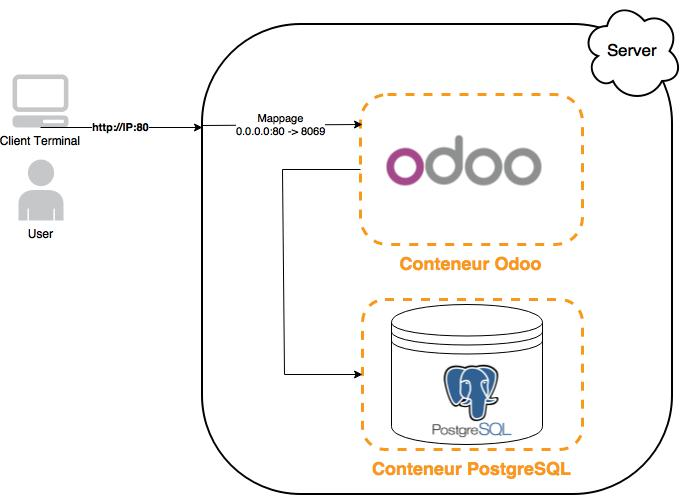
\includegraphics [scale=0.5]{biblio/odoo.jpg}
	\caption{Odoo sous Docker}
	\label{fig:}
	\end{figure}

\section*{Environnement technique}
	
	On va partir d'un serveur Ubuntu 14.04-64 bits avec Docker installé (L'installation ne sera pas détaillé), ou de préférence, un serveur CoreOS où Docker est déja inclut avec ce système d'éxploitation. A noter que Docker nécéssite un linux 64 bits avec un noyau >= 3.8.


\section*{Installation de PostgreSQL}

	Odoo a besoin d'un serveur de base de donnée PostgreSQL, la commande suivante permet de l'installer:

	\begin{lstlisting}[caption=Installation de PostgreSQL]
		$ docker run -d -e POSTGRES_USER=odoo -e POSTGRES_PASSWORD=odoo --name db postgres
	\end{lstlisting}




\section*{Installation d'Odoo}

	L'installation d'Odoo se fait grâce à la commande suivante:
	\begin{lstlisting}[language=bash,caption=Installation d'Odoo]
		$ docker run -p 80:8069 --name odoo --link db:db -t odoo
	\end{lstlisting}

	En quelques secondes, on pu lancer le service Odoo prêt à être utilisé, personnalisé, et éventuellement porté vers un autre serveur. Pour accéder au service il suffit de taper dans le navigateur:

	\begin{lstlisting}[language=bash]
		http://IP_SERVEUR:80
	\end{lstlisting}

	




\chapter{Docker-compose}

	On va réaliser l'installation détaillé dans \emph{l'Annexe A} avec l'outil \emph{Docker-compose}. Cet outil permet de définir dans un fichier YAML* l'architecture de l'application. Enfin, on peut faire des manipulation (démarrage, redémarrage, arrêt) sur toute l'architecture comme si c'était un seul service.

	\begin{lstlisting}[language=bash,caption=Installation d'Odoo avec Docker-compose]
		odoo:
	  		image: odoo
		  	links:
		   		- db
		  	ports:
		   		- "80:8069"
		db:
		  	image: postgres
		  	environment:
  				- POSTGRES_USER: odoo
  				- POSTGRES_PASSWORD: odoo
	\end{lstlisting}

	\begin{lstlisting}[language=bash,caption=Lancement d'Odoo avec Docker-compose]
		$ docker-compose up -d
	\end{lstlisting}


\chapter{Installation du superviseur}
	
	Voici les fichiers d'installations de cAdvisor, InfluxDB, Heapster et Grafana. On va les charger dans le cluster puis les installer un à la suite de l'autre.

	\begin{lstlisting}[language=,caption=cadvisor.service]
		[Unit]
		After=docker.service
		Requires=docker.service
		[Service]
		Restart=always
		ExecStartPre=/usr/bin/docker pull google/cadvisor:latest
		ExecStartPre=-/bin/bash -c "docker inspect cadvisor >/dev/null 2>&1 && docker rm -f cadvisor || true"
		ExecStart=/usr/bin/docker run --volume=/var/run:/var/run:rw --volume=/sys/fs/cgroup/:/sys/fs/cgroup:ro --volume=/var/lib/docker/:/var/lib/docker:ro --publish=8080:8080 --name=cadvisor google/cadvisor:latest
		ExecStop=/usr/bin/docker rm -f cadvisor
		[X-Fleet]
		Global=true

	\end{lstlisting}

	\begin{lstlisting}[language=,caption=influxdb.service]
		[Unit]
		After=docker.service
		Requires=docker.service
		Rquires=docker_configs.mount
		[Service]
		ExecStartPre=-/usr/bin/docker kill influxdb
		ExecStartPre=-/usr/bin/docker rm influxdb
		ExecStartPre=/usr/bin/docker pull kubernetes/heapster_influxdb:v0.3
		ExecStart=/usr/bin/docker run -p 8083:8083 -p 8086:8086 -v /data/influxdb:/data --hostname="influxdb" --name influxdb kubernetes/heapster_influxdb:v0.3
		ExecStop=/usr/bin/docker stop nodejscluster
		TimeoutStartSec=0
		Restart=always
		RestartSec=5s

	\end{lstlisting}

	\begin{lstlisting}[language=,caption=heapster.service]
		[Unit]
		After=docker.service
		After=influxdb.service
		Requires=docker.service
		Requires=influxdb.service
		[Service]
		TimeoutStartSec=0
		ExecStartPre=-/usr/bin/docker kill heapster
		ExecStartPre=-/usr/bin/docker rm heapster
		ExecStart=/bin/bash -c "HOST_IP=`getent hosts %H|/usr/bin/cut -d\" \" -f1`; /usr/bin/docker run --name heapster --link influxdb:influxdb kubernetes/heapster:v0.13.0 --source=\"cadvisor:coreos?fleetEndpoint=http://$HOST_IP:4001&cadvisorPort=8080\" --sink='influxdb:http://influxdb:8086'"
		Restart=always
		RestartSec=5
		ExecStop=/usr/bin/docker stop heapster
		[X-Fleet]
		X-ConditionMachineOf=influxdb.service
	\end{lstlisting}

	\begin{lstlisting}[language=,caption=grafana.service]
		[Unit]
		After=docker.service
		After=influxdb.service
		Requires=docker.service
		Requires=influxdb.service
		[Service]
		TimeoutStartSec=0
		ExecStartPre=-/usr/bin/docker kill grafana
		ExecStartPre=-/usr/bin/docker rm grafana
		ExecStart=/usr/bin/docker run --name=grafana --link influxdb:influxdb -p 8090:8080 -e INFLUXDB_HOST=influxdb kubernetes/heapster_grafana:v0.7
		Restart=always
		RestartSec=5
		ExecStop=/usr/bin/docker stop grafana
		[X-Fleet]
		X-ConditionMachineOf=influxdb.service
	\end{lstlisting}	

	\begin{lstlisting}[language=bash,caption=Lancement des services]
		$ ssh core@104.154.75.6 
		$ fleetctl load cadvisor.service
		$ fleetctl start cadvisor.service
	\end{lstlisting}